% Formal Fock space, ladder operators, raising exponentials and the Bargmann picture.
% The bosonic matrix product states built on it: Tjoa and Cirac, arXiv:2607.28753.
\providecommand{\ket}[1]{\lvert #1\rangle}
\providecommand{\bra}[1]{\langle #1\rvert}
\providecommand{\Tr}{\operatorname{Tr}}
\providecommand{\N}{\mathbb N}
\providecommand{\Fock}{\mathcal F}
\providecommand{\Barg}{\mathfrak B}
\providecommand{\coef}[2]{[z^{#1}]\,#2}
\clearpage
\section{The formal Fock space and the Bargmann picture}\label{sec:fock}
The number basis of a bosonic Fock space labels vectors by occupation numbers. Allowing all
coefficient families, with no summability condition, gives a space on which the creation
operators and the exponentials of operators that raise the particle number act exactly, one
coefficient at a time. This section develops that formal Fock space, the canonical
commutation relations on it, the exponential law for raising operators, and the Bargmann
picture, in which creation and annihilation become multiplication by and differentiation in
formal variables. The exponentials of the Gaussian-augmented bosonic matrix product states of
Tjoa and Cirac~\cite{tjoacirac} are of this kind. \reva{Those states are a
different construction from the Gaussian matrix product states whose covariance matrices are
built by contraction in Sections~\ref{sec:contraction}--\ref{sec:products}; these notes do not
yet relate the two.}

\medskip
\noindent\textbf{Notation for this section.}
\begin{center}
\begin{tabular}{ll}
$\iota$ & a set of modes\\
$n=(n_i)_{i\in\iota}$ & a multi-index of occupation numbers, finitely many nonzero\\
$m$ & an occupation number of a single mode\\
$e_i$ & the multi-index with a single $1$ at $i$\\
$\lvert n\rvert=\sum_i n_i$ & total particle number of $n$\\
$n!=\prod_i n_i!$ & factorial of a multi-index\\
$\ket n$ & number state (Definition~\ref{def:fock-space})\\
$\Fock(\iota,R)$ & formal Fock space with coefficients in $R$ (Definition~\ref{def:fock-space})\\
$\mathfrak h$, $\Gamma_s(\mathfrak h)$ & for finite $\iota$, the one-particle space $\C^\iota$ and its Fock space\\
$a_i^\dagger,\ a_i$ & creation and annihilation operators (Definition~\ref{def:fock-ladder})\\
$T$, $T'$, $e^T$ & raising operators and their exponential (Definition~\ref{def:fock-raising})\\
$R[[z]]$, $\partial_j$ & formal power series in $(z_i)_{i\in\iota}$ over $R$; partial derivative\\
$\coef nf$ & coefficient of $z^n=\prod_iz_i^{n_i}$ in $f\in R[[z]]$\\
$\Barg$ & Bargmann map (Definition~\ref{def:fock-bargmann})\\
\end{tabular}
\end{center}
\reva{In this section $R$ is a $\C$-algebra, $X\in R$, $n$ a multi-index, $W$ a word in the
ladder operators, $T$ a raising operator, $p\ge1$ an exponent, $z$ the formal variables and
$\Lambda$ a bound on particle numbers; letters shared with
Sections~\ref{sec:covariance}--\ref{sec:products} do not carry their meanings from there.}

\subsection{The formal Fock space}

Throughout, $R$ is a $\C$-algebra: a ring together with a ring homomorphism from $\C$ into
its centre. The two cases used later are $R=\C$ (states) and $R=M_\beta(\C)$, the complex
matrices indexed by a finite set $\beta$ (vectors that carry a matrix index); for $\beta$
empty, $M_\beta(\C)$ is the zero ring, which is allowed.

\begin{definition}[Formal Fock space]\label{def:fock-space}
$\Fock(\iota,R)$ is the set of all functions $\psi$ from multi-indices to $R$, with
pointwise addition and scalar multiplication; $\psi$ is read as $\sum_n\psi(n)\ket n$.
The number state $c\ket n$ has coefficient $c$ at $n$ and $0$ elsewhere, and $\ket0$ is
the vacuum. A vector $\psi$ \emph{vanishes below $k$} if $\psi(n)=0$ whenever
$\lvert n\rvert<k$.
\end{definition}

No summability is imposed. For finite $\iota$ and the one-particle space $\mathfrak
h=\C^\iota$ with its standard orthonormal basis, the $k$-particle space
$\otimes_s^k\mathfrak h$ has as orthonormal basis the number states $\ket n$ with
$\lvert n\rvert=k$, so that, sector by sector,
\[
 \Gamma_{\mathrm{fin}}(\mathfrak h)=\bigoplus_{k}\otimes_s^k\mathfrak h\ \subset\
 \Gamma_s(\mathfrak h)=\overline{\bigoplus_{k}}\,\otimes_s^k\mathfrak h\ \subset\
 \prod_{k}\otimes_s^k\mathfrak h=\Fock(\iota,\C):
\]
the finite-particle space, the bosonic Fock space of~\cite{dg,br} (the Hilbert direct sum,
that is, the square-summable families) and the full product. \reva{$\Gamma_s(\mathfrak h)$
is recalled from~\cite{dg,br}; it is not constructed in these notes}\revs{, nor are second
quantization, the Fock representation of the CCR algebra, or the identification of
$\Gamma_s(\mathfrak h)$ with $L^2(\R^\iota)$ through the Hermite functions that would join this
section to Sections~\ref{sec:covariance}--\ref{sec:products}}. For a single mode, the vector with
coefficients $\sqrt{(2k)!}/k!$ at $\ket{2k}$ and $0$ at odd occupations lies in
$\Fock(\{1\},\C)$ but not in $\Gamma_s$, since $(2k)!/(k!)^2\ge1$. After
Definition~\ref{def:fock-raising} it is $e^{(a^\dagger)^2}\ket0$.

\begin{definition}[Ladder operators and left multiplication]\label{def:fock-ladder}
For $i\in\iota$, the creation and annihilation operators are the $\C$-linear maps
\[
 (a_i^\dagger\psi)(n)=\begin{cases}\sqrt{n_i}\,\psi(n-e_i),&n_i\ge1,\\0,&n_i=0,\end{cases}
 \qquad (a_i\psi)(n)=\sqrt{n_i+1}\,\psi(n+e_i).
\]
For $X\in R$, $X\psi$ is the vector with coefficients $X\psi(n)$. For a word $W$ in the
ladder operators, $X\otimes W$ denotes the composite $XW$; the two factors commute, since a
ladder word multiplies each coefficient by complex scalars and moves it, while $X$
multiplies it on the left, and complex scalars are central in $R$.
\end{definition}

On number states these are the formulas $a_i^\dagger\ket n=\sqrt{n_i+1}\ket{n+e_i}$ and
$a_i\ket n=\sqrt{n_i}\ket{n-e_i}$. On $\Gamma_s(\mathfrak h)$ the creation and annihilation
operators of~\cite{dg} are $a^*(h)=\sum_ih_ia_i^\dagger$ and $a(h)=\sum_i\overline{h_i}\,a_i$
for $h\in\mathfrak h$. Each coefficient of $a_i^\dagger\psi$ or $a_i\psi$ involves a single
coefficient of $\psi$, so both operators are defined on the whole formal Fock space.

\begin{theorem}[Canonical commutation relations]\label{thm:fock-ccr}
On all of $\Fock(\iota,R)$: $[a_i,a_j^\dagger]=\delta_{ij}$, $[a_i,a_j]=0$ and
$[a_i^\dagger,a_j^\dagger]=0$.
\end{theorem}

\begin{proof}
We check the identities coefficientwise.
\begin{enumerate}
\item[(a)] For $i=j$: $(a_ia_i^\dagger\psi)(n)=\sqrt{n_i+1}\sqrt{n_i+1}\,\psi(n)$ and
$(a_i^\dagger a_i\psi)(n)=\sqrt{n_i}\sqrt{n_i}\,\psi(n)$, the second being $0$ when $n_i=0$.
The difference is $\psi(n)$.
\item[(b)] For $i\ne j$, both orders give $\sqrt{n_j}\sqrt{n_i+1}\,\psi(n+e_i-e_j)$ when
$n_j\ge1$, and $0$ otherwise, because shifting $n_i$ does not change $n_j$.
\item[(c)] For $i\ne j$, $a_ia_j$ and $a_ja_i$ both multiply $\psi(n+e_i+e_j)$ by
$\sqrt{n_i+1}\sqrt{n_j+1}$; $a_i^\dagger a_j^\dagger$ and $a_j^\dagger a_i^\dagger$ both
multiply $\psi(n-e_i-e_j)$ by $\sqrt{n_i}\sqrt{n_j}$ when $n_i,n_j\ge1$, and give $0$
otherwise. For $i=j$ there is nothing to prove.\qedhere
\end{enumerate}
\end{proof}

\reva{Since $a_i^\dagger(c\ket n)=\sqrt{n_i+1}\,c\ket{n+e_i}$ and the creation operators
commute, $\prod_i(a_i^\dagger)^{n_i}(c\ket0)=\sqrt{n!}\,c\ket n$, the product running over the
finitely many $i$ with $n_i\ne0$. So $\ket n=\prod_i(a_i^\dagger)^{n_i}\ket0/\sqrt{n!}$, as
usual.}

\subsection{Raising operators and their exponentials}

Operators that raise the particle number have exponential series that are finite at each
coefficient.

\begin{definition}[Raising operator and its exponential]\label{def:fock-raising}
A $\C$-linear map $T$ on $\Fock(\iota,R)$ is \emph{raising} (short for order-raising) if, for
every $k$, $T\psi$
vanishes below $k+1$ whenever $\psi$ vanishes below $k$. For raising $T$,
\[
 (e^T\psi)(n)=\sum_{r=0}^{\lvert n\rvert}\frac{(T^r\psi)(n)}{r!}.
\]
\end{definition}

\begin{lemma}\label{lem:fock-raising}
Let $T$ and $T'$ be raising.
\begin{enumerate}
\item[(a)] If $T_1,\ldots,T_r$ are raising and $\psi$ vanishes below $k$, then
$T_1\cdots T_r\psi$ vanishes below $k+r$. In particular $(T^r\psi)(n)=0$ for
$r>\lvert n\rvert$, and $(e^T\psi)(n)=\sum_{r=0}^{\Lambda}(T^r\psi)(n)/r!$ for every
$\Lambda\ge\lvert n\rvert$.
\item[(b)] $(T\psi)(n)$ depends only on the coefficients $\psi(n')$ with
$\lvert n'\rvert<\lvert n\rvert$.
\item[(c)] $T+T'$, $TT'$ and $cT$ ($c\in\C$) are raising; so are $a_i^\dagger$ and, for
$X\in R$ and $p\ge1$, $X(a_i^\dagger)^p$.
\end{enumerate}
\end{lemma}

\begin{proof}
\begin{enumerate}
\item[(a)] Apply the definition to $T_r$, then $T_{r-1}$, and so on; each step raises the
bound by one. Every $\psi$ vanishes below $0$.
\item[(b)] If $\psi$ and $\psi'$ agree in degrees below $\lvert n\rvert$, then $\psi-\psi'$
vanishes below $\lvert n\rvert$, so $T(\psi-\psi')$ vanishes below $\lvert n\rvert+1$, in
particular at $n$.
\item[(c)] The first three claims follow from the definition. $(a_i^\dagger\psi)(n)$ is a
multiple of $\psi(n-e_i)$ and $\lvert n-e_i\rvert=\lvert n\rvert-1$, so $a_i^\dagger$ is
raising; hence so is $(a_i^\dagger)^p$ for $p\ge1$, and left multiplication by $X$
preserves vanishing below $k$.\qedhere
\end{enumerate}
\end{proof}

\reva{We define the exponential by the finite sum of Definition~\ref{def:fock-raising},
not as a limit, so no topology on $\Fock(\iota,R)$ is needed.} By Lemma~\ref{lem:fock-raising}(a) this is the operator series
$\sum_rT^r/r!$ itself: at every coefficient the partial sums are constant from
$r=\lvert n\rvert$ on. When the series converges in $\Gamma_s(\mathfrak h)$, its limit has
these coefficients, since convergence there implies convergence of each coefficient.

\begin{figure}[ht]
\centering
\revb{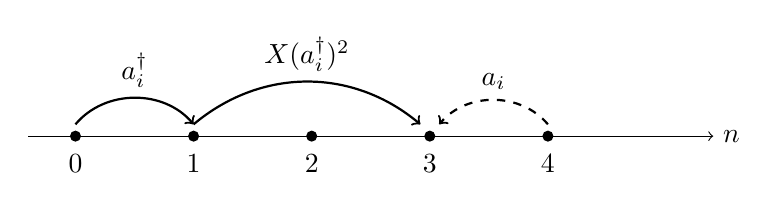
\begin{tikzpicture}[x=1.5cm]
 \draw[->] (-0.4,0) -- (5.4,0) node[right] {$\lvert n\rvert$};
 \foreach \k in {0,...,4} \fill (\k,0) circle (2pt) node[below=3pt] {$\k$};
 \draw[->,thick] (0,0.15) to[bend left=50] node[above] {$a_i^\dagger$} (1,0.15);
 \draw[->,thick] (1,0.15) to[bend left=40] node[above] {$X(a_i^\dagger)^2$} (2.92,0.15);
 \draw[->,thick,dashed] (4,0.15) to[bend right=50] node[above] {$a_i$} (3.08,0.15);
\end{tikzpicture}
\caption{Raising maps (solid) move every coefficient to strictly higher particle number; the
annihilation operator (dashed) moves it down. Hence the coefficient of $e^T\psi$ at particle
number $k$ receives only the terms $T^r\psi$ with $r\le k$: the finite sum of
Definition~\ref{def:fock-raising}.}\label{fig:fock-grading}}
\end{figure}

\begin{theorem}[Exponential law]\label{thm:fock-explaw}
If $T$ and $T'$ are raising and $TT'=T'T$, then $e^{T+T'}=e^Te^{T'}$.
\end{theorem}

\begin{proof}
\reva{By Lemma~\ref{lem:fock-raising}(c), $T+T'$ is raising, so both sides are
defined; likewise $T^r$ is raising for $r\ge1$, which is used below.} The coefficient of $e^Te^{T'}\psi$ at
$n$ reduces to a finite double sum, which the binomial theorem collapses. Fix $n$ and $\psi$,
and put $\Lambda=\lvert n\rvert$. By Lemma~\ref{lem:fock-raising}(a), $e^{T'}\psi$ agrees in all
degrees $\le\Lambda$ with $\sum_{t=0}^\Lambda T'^t\psi/t!$. By Lemma~\ref{lem:fock-raising}(b),
applied to the raising map $T^r$ for $r\ge1$ (and trivially for $r=0$),
\[
 (e^Te^{T'}\psi)(n)=\sum_{r=0}^\Lambda\sum_{t=0}^\Lambda\frac{(T^rT'^t\psi)(n)}{r!\,t!}
 =\sum_{k=0}^\Lambda\frac1{k!}\sum_{r+t=k}\binom kr(T^rT'^t\psi)(n)
 =\sum_{k=0}^\Lambda\frac{((T+T')^k\psi)(n)}{k!}.
\]
We dropped the terms with $r+t>\Lambda$ because $T^rT'^t$ is a product of $r+t$ raising maps and
therefore, by Lemma~\ref{lem:fock-raising}(a), vanishes at $n$; the last step is the
binomial theorem for commuting $T$ and $T'$. The right side is $(e^{T+T'}\psi)(n)$.
\end{proof}

For matrices the same identity rests on absolute convergence of the double series. Here the
grading by particle number replaces it. \reva{Without the raising hypothesis the finite sum of
Definition~\ref{def:fock-raising} need not agree with the series $\sum_r(T^r\psi)(n)/r!$, and
the series need not converge. For the annihilation operator $a$ of a single mode and
$\psi=\ket1$, the finite sum at $n=0$ is $\psi(0)=0$, while the series gives
$(a\psi)(0)=1$. For $\psi(m)=m!$, the series $\sum_k(a^k\psi)(0)/k!=\sum_k\sqrt{k!}$
diverges.}

\subsection{The Bargmann picture}

\reva{$R[[z]]$ is the set of all functions $f$ from multi-indices to $R$, written
$f=\sum_n\coef nf\,z^n$, with the Cauchy product
$\coef n{(fg)}=\sum_{n'+n''=n}\coef{n'}f\,\coef{n''}g$, a finite sum.} For $f\in R[[z]]$, we define the partial derivative coefficientwise by
$\coef n{(\partial_jf)}=(n_j+1)\,\coef{n+e_j}f$; for $R=\C$ it is the usual derivative of
formal power series.

\begin{definition}[Bargmann map]\label{def:fock-bargmann}
$\Barg:\Fock(\iota,R)\to R[[z]]$ is given by $\coef n{\Barg\psi}=\psi(n)/\sqrt{n!}$.
It is a $\C$-linear bijection, with inverse $\psi(n)=\sqrt{n!}\,\coef nf$.
\end{definition}

Thus $\Barg\ket n=z^n/\sqrt{n!}$, which for finite $\iota$ is the orthonormal basis of
Bargmann's space of entire functions~\cite{bargmann}. So $\Barg$ maps $\Gamma_s(\mathfrak h)$
onto the Taylor series of the Bargmann space, and the formal Fock space onto all of $R[[z]]$,
including, \reva{for a single mode and $R=\C$,} series such as $\sum_mm!\,z^m=\Barg\psi$,
$\psi(m)=m!\sqrt{m!}$, with radius of convergence $0$. A vector $\psi$ vanishes below $k$
exactly when $\Barg\psi$ has order at least $k$ (no monomial of total degree below $k$), so a
raising map raises the order of power
series by at least one; hence the name.

\begin{lemma}\label{lem:fock-factorial}
If $n_j\ge1$, then $n!=n_j\,(n-e_j)!$.
\end{lemma}

\begin{proof}
$n$ and $n-e_j$ differ only in the $j$-th entry, and $n_j!=n_j\,(n_j-1)!$.
\end{proof}

\begin{lemma}\label{lem:fock-shift}
For every $f\in R[[z]]$: $\coef n{(z_j^mf)}=\coef{n-me_j}f$ if $m\le n_j$, and $0$ if
$m>n_j$.
\end{lemma}

\begin{proof}
This is the coefficient formula for multiplication by the monomial $z_j^m$; it holds for
non-commutative $R$ because $z_j^m$ has a scalar coefficient.
\end{proof}

\begin{theorem}[Intertwining]\label{thm:fock-bargmann}
For every $\psi\in\Fock(\iota,R)$ and $X\in R$:
\begin{enumerate}
\item[(a)] $\Barg(a_j^\dagger\psi)=z_j\,\Barg\psi$;
\item[(b)] $\Barg(a_j\psi)=\partial_j\Barg\psi$;
\item[(c)] $\Barg(X\psi)=X\,\Barg\psi$;
\item[(d)] $\Barg\ket0=1$.
\end{enumerate}
\end{theorem}

\begin{proof}
\begin{enumerate}
\item[(a)] At $n$ with $n_j\ge1$, Lemma~\ref{lem:fock-factorial} gives
\[
 \coef n{\Barg(a_j^\dagger\psi)}=\frac{\sqrt{n_j}\,\psi(n-e_j)}{\sqrt{n!}}
 =\frac{\psi(n-e_j)}{\sqrt{(n-e_j)!}},
\]
which is $\coef n{(z_j\Barg\psi)}$ by Lemma~\ref{lem:fock-shift}. If $n_j=0$, both sides
vanish.
\item[(b)] By Lemma~\ref{lem:fock-factorial} at $n+e_j$,
\[
 \coef n{\Barg(a_j\psi)}=\frac{\sqrt{n_j+1}\,\psi(n+e_j)}{\sqrt{n!}}
 =(n_j+1)\,\frac{\psi(n+e_j)}{\sqrt{(n+e_j)!}},
\]
\reva{which is $\coef n{(\partial_j\Barg\psi)}$.}
\item[(c)] $1/\sqrt{n!}$ is a complex scalar and commutes with $X$.
\item[(d)] $\coef0{\Barg\ket0}=1/\sqrt{0!}=1$, and all other coefficients vanish.\qedhere
\end{enumerate}
\end{proof}

For $X\in R$, $j\in\iota$ and $p\ge1$, the formal exponential $e^{Xz_j^p}$ is the series
$\sum_{k\ge0}X^kz_j^{pk}/k!$ in the single variable $z_j$.

\begin{theorem}[Exponentials in the Bargmann picture]\label{thm:fock-exp-bargmann}
\reva{For $X\in R$, $j\in\iota$, $p\ge1$ and every $\psi\in\Fock(\iota,R)$:}
$\Barg\bigl(e^{X\otimes(a_j^\dagger)^p}\psi\bigr)=e^{Xz_j^p}\;\Barg\psi$.
\end{theorem}

\begin{proof}
Write $T=X(a_j^\dagger)^p$ and $f=\Barg\psi$. By Theorem~\ref{thm:fock-bargmann}, and since
$z_j$ commutes with every series, induction on $k$ gives $\Barg(T^k\psi)=X^kz_j^{pk}f$.
Fix $n$. Then
\[
 \coef n{\Barg(e^T\psi)}=\sum_{k=0}^{\lvert n\rvert}\frac1{k!}\coef n{(X^kz_j^{pk}f)}.
\]
The coefficient of a product $Pf$ at $n$ involves only the coefficients of $P$ at
multi-indices $n'\le n$. For such $n'$, the coefficient of $e^{Xz_j^p}$ at $n'$ equals that of
the polynomial $\sum_{k\le\lvert n\rvert}X^kz_j^{pk}/k!$: a term with $k>\lvert n\rvert$
sits at a multi-index of total degree $pk\ge k>\lvert n\rvert\ge\lvert n'\rvert$. Hence
$\coef n{(e^{Xz_j^p}f)}$ is the same finite sum.
\end{proof}

The truncation in Definition~\ref{def:fock-raising} therefore cuts only terms whose
coefficient at $n$ vanishes.

